\documentclass[journal]{IEEEtran}

\usepackage{graphicx}
\usepackage{booktabs}
\usepackage{array}
\usepackage{amsmath,amssymb}
\usepackage{url}
\usepackage{microtype}
\usepackage{tikz}
\usetikzlibrary{arrows.meta,positioning,calc}
\usepackage[hidelinks]{hyperref}
\hypersetup{
  pdftitle={Beyond Reconnection: Measuring Recovery Observables and Replay-Induced Continuity Gaps in MQTT Telemetry},
  pdfauthor={Ahmed Ayoub},
  pdfsubject={Experimental recovery observables for MQTT telemetry},
  pdfkeywords={MQTT, telemetry recovery, data durability, backlog replay, receiver reconciliation, IoT testbeds}
}

% WellPulse IEEE Revival -- R7b source skeleton.
% NEW SOURCE IDENTITY. Does not overwrite rejected TNSM release.
% Governing science: experiments/WP-RT01/R6_INTEGRATED_SCIENTIFIC_ADJUDICATION.md

\begin{document}

\title{Beyond Reconnection: Measuring Recovery Observables and Replay-Induced Continuity Gaps in MQTT Telemetry}

\author{Ahmed Ayoub%
\thanks{A. Ayoub is with the Computer Systems Engineering Department, Faculty of Engineering, October University for Modern Sciences and Arts (MSA University), 6th of October City, 12451, Egypt (e-mail: aelsayedo@msa.edu.eg; ORCID: 0009-0004-7895-3191).}}

\maketitle

\begin{abstract}
Telemetry recovery is often summarized by a single reconnect or catch-up time, although network restoration, MQTT session restoration, broker-side QoS-1 acknowledgement closure, receiver-side historical completion, live-data continuity, and stale-record carryover are different observables. This study applies an operational measurement discipline that separates these states to MQTT telemetry on FIT IoT-LAB and POWDER. In the tested W1 implementation, serialized backlog replay preserved eventual 10,000/10,000 receiver completeness but repeatedly suspended new record generation. Six historical FIT runs showed sequence-5000-to-5001 gaps of 68.785--70.264~s (mean 69.217~s); three prospective scored runs showed 74.798--76.308~s (mean 75.438~s). These measurements quantify the magnitude and repeatability of a continuity cost implied by the tested serialized replay order. The prospective runs directly instrumented sender PUBACK closure and receiver completion, but 0/3 produced either a causal witness or a clock-resolved positive M2-to-M3 separation, so that interval remains unresolved. A POWDER trace independently exhibited stale carryover after restoration. The measurement discipline prevents sender-side acknowledgement closure from being mislabeled as receiver completion while keeping replay-associated continuity evidence separate from the unresolved M2-to-M3 question.
\end{abstract}

\begin{IEEEkeywords}
MQTT, telemetry recovery, data durability, backlog replay, receiver reconciliation, fault injection, IoT testbeds.
\end{IEEEkeywords}

\section{Introduction}
\label{sec:introduction}

A telemetry system can become reachable before all of the state that matters to the application is restored. MQTT itself exposes several different events during recovery: a network path may respond, an MQTT session may reconnect, a broker may acknowledge a QoS-1 publish, a subscriber may eventually receive all required historical records, and the source may or may not continue generating current records while old data are replayed. Treating any one of these events as a generic recovery time risks mixing different system states and different operational questions.

This distinction matters most when durability is implemented by buffering historical records during an outage and replaying them after connectivity returns. Persistence can preserve eventual completeness, yet the replay policy can still affect continuity of current data generation. Conversely, a lower-layer path can remain available while the application service is unavailable, and a receiver can observe stale historical records after newer records have already arrived. These cases motivate measurement that names the failure domain, the endpoint being observed, and the evidence required to close each recovery state.

This study therefore applies an \emph{operational recovery-measurement discipline}, not a new MQTT persistence or failover architecture and not a claim that the labels M0--M5 are novel by themselves. The discipline separates six observables: network-path restoration (M0), MQTT-session restoration (M1), sender-to-broker QoS-1 acknowledgement closure (M2), receiver-side historical-state completion (M3), live-data continuity (M4), and receiver ordering/stale carryover (M5). Its purpose is evidentiary: each endpoint has a declared authority and claim ceiling, so sender-side progress is not silently relabeled as receiver completion. M2 and M3 therefore remain different system states even when a measurable positive time separation between them cannot be resolved.

The measurement discipline is applied to two non-pooled evidence classes. FIT IoT-LAB provides controlled broker/process disruption and repeated run-level measurements of record survival and serialized W1 replay. POWDER provides physical/network/service failure-domain observations, including exact, censored, and upper-bounded recovery measurements. A prospective FIT Stage-A campaign then directly instruments M2 and M3 to test a claim that the historical campaign could not resolve.

\subsection{Research Questions}
The study is organized around four bounded research questions:
\begin{enumerate}
    \item[\textbf{RQ1}] Which experimentally observable endpoints are required to distinguish network-path restoration, MQTT-session restoration, broker-side QoS-1 acknowledgement closure, receiver-side historical completion, live-data continuity, and receiver-side stale carryover?
    \item[\textbf{RQ2}] Under the tested serialized W1 backlog-replay implementation, what live-generation discontinuity is observed in the historical and prospective FIT IoT-LAB campaigns?
    \item[\textbf{RQ3}] When M2 and M3 are directly instrumented prospectively, does the qualified evidence resolve a positive M2-to-M3 separation under the frozen causal-witness and clock-uncertainty rules?
    \item[\textbf{RQ4}] What complementary, bounded evidence does POWDER provide about failure-domain-specific recovery and receiver-side stale carryover without pooling the two testbeds?
\end{enumerate}

\subsection{Contributions}
The contribution set is deliberately narrower than a new recovery architecture or a new taxonomy:
\begin{enumerate}
    \item[\textbf{A1}] \textbf{Operational recovery-measurement discipline.} A measurement procedure that assigns evidence authority and a claim ceiling to M0--M5 so reconnect, session restoration, PUBACK closure, receiver completion, continuity, and ordering are not treated as interchangeable evidence. Its concrete validation is the reclassification of the historical sender-side backlog endpoint and the prospective M2/M3 adjudication.
    \item[\textbf{A2}] \textbf{Measured W1 replay consequence.} Across separate historical and prospective FIT campaigns, the experiments quantify the magnitude and repeatability of a code-path-implied continuity cost: the tested serialized replay order suspends new record generation for tens of seconds while eventual receiver completeness is preserved.
    \item[\textbf{A3}] \textbf{Complementary cross-environment evidence without pooling.} FIT provides implementation-specific replay evidence; POWDER provides bounded physical failure-domain and stale-carryover evidence. The environments answer different measurement questions and are not treated as replications of one common effect.
    \item[\textbf{A4}] \textbf{Prospective endpoint adjudication.} Direct M2/M3 instrumentation produced 0/3 positive results and 3/3 UNRESOLVED outcomes, constraining the claim ceiling rather than being converted into a favorable recovery result.
\end{enumerate}

The remainder of the paper is organized as follows. Section~\ref{sec:related} positions the measurement problem against MQTT reliability, robustness, end-to-end confirmation, high-availability recovery, and freshness/reconstruction prior art. Section~\ref{sec:protocol} defines M0--M5 and the FIT and POWDER protocols. Section~\ref{sec:results} reports the historical FIT, prospective FIT, and POWDER evidence without pooling. Section~\ref{sec:discussion} interprets the measured W1 replay consequence and its service-management implications. Section~\ref{sec:threats} states the principal validity limits, Section~\ref{sec:repro} records the evidence-preservation boundary, and the final section summarizes the bounded conclusions.

\section{Related Work and Claim Boundary}
\label{sec:related}

\subsection{MQTT QoS semantics and end-to-end confirmation}

MQTT QoS semantics and broker-mediated acknowledgements are well established. Nawaz et al. formally model the QoS levels and their delivery semantics, reinforcing that protocol-level guarantees must be interpreted according to the MQTT interaction being acknowledged \cite{nawaz2019}. MQTT itself defines publisher--broker protocol exchanges, whereas publisher knowledge of downstream application persistence requires additional evidence \cite{mqtt5}.

Subscriber- or application-level confirmation is also prior art. Im and Lim's E-MQTT augments MQTT with subscriber responses so that publishers can determine when one or more subscribers have received a message \cite{emqtt}. More recently, Mohammed et al. proposed MQTT monitoring architectures with disk-backed persistence and application/database-level acknowledgements beyond broker QoS in two 2026 studies \cite{mohammed2026resilient,mohammed2026scalable}. These works directly preclude any claim that application-level acknowledgement, disk-backed persistence, or end-to-end durability confirmation is introduced here. The present study instead treats receiver reconciliation as measurement evidence and asks what can be concluded from distinct recovery endpoints under disruption.

\subsection{Broker failure, distributed brokers, and implementation variability}

Broker resilience and broker-distribution mechanisms are likewise established. Chen et al. study broker-crash handling by rerouting topic-session flows to another broker so communication can continue after a broker failure \cite{chen2020}. Kamoun et al. review and extend distributed MQTT broker architectures in which broker functionality is moved toward fog, edge, or mist nodes, noting availability and performance motivations for avoiding a centralized broker bottleneck \cite{kamoun2024}. These mechanisms mean that broker failover, broker substitution, and distributed-broker availability are prior art rather than contributions of this study.

MQTT implementations also differ in behavior. Sochor et al. evaluate compatibility across multiple MQTT brokers and versions and report behavior differences that matter when replacing or upgrading brokers \cite{sochor2021}. The present experiments therefore do not assume that results from one client/broker/software path characterize MQTT implementations in general.

\subsection{Robustness, stress testing, and reliability trade-offs}

Fault injection and robustness evaluation of MQTT-based IoT systems are established topics. Jesus, Lins, and Laranjeiro inject faults into MQTT-carried messages to activate residual application-level failures and assess robustness across case studies \cite{jesus2025}. Gaspar et al. stress-test MQTT reliability under practical communication conditions and characterize the cost of reliability choices \cite{gaspar2026}. This study therefore does not claim novelty from fault injection, stress testing, packet loss, or MQTT reliability measurement. Its narrower question is how recovery evidence should be separated by endpoint and how an implementation-specific replay policy affects current-data continuity while preserving eventual state.

\subsection{Layered recovery, high availability, and data continuity}

Layered recovery is not new. Neagu et al. evaluate a high-availability edge architecture using separate network-layer, application-layer, and data-continuity measurements, including VIP failover, MQTT/service restoration, and message loss \cite{neagu2026}. Together with broker-failover and distributed-broker work \cite{chen2020,kamoun2024}, this directly precludes a claim that merely separating path, service, or data recovery is itself novel. The present study instead applies a finer evidence discipline to receiver-reconciled state, source-generation continuity, and same-receiver ordering, while preserving exact, censored, and upper-bound observations as different evidence types.

\subsection{Freshness versus historical reconstruction}

The tension between current-state freshness and reconstruction of historical state is also recognized outside MQTT. Kang et al. formulate a remote-tracking scheduler that explicitly trades current-state freshness against historical reconstruction queue length \cite{kang2026}. Consequently, a live-versus-history scheduling trade-off is not claimed as a new concept here. The FIT evidence is narrower: it quantifies the repeatability and magnitude of a continuity cost that is implied by the tested W1 implementation's serialized replay order.

\subsection{Retained gap}

The literature now covers MQTT QoS semantics, subscriber/application confirmation, disk-backed persistence with application-level acknowledgement, broker substitution and distributed brokers, robustness/fault injection, broker compatibility, reliability stress testing, layered high-availability recovery, and freshness-versus-reconstruction scheduling. The retained gap is therefore not architectural firstness, end-to-end acknowledgement novelty, or the novelty of naming recovery layers.

The remaining contribution is an operational measurement discipline that assigns each recovery endpoint an evidence authority and claim ceiling, then demonstrates why that discipline matters in the present evidence set. The historical FIT campaign provides the concrete correction case: a sender-side backlog/PUBACK endpoint that had previously been interpreted as receiver completion is reclassified once M2 and M3 are separated. The prospective campaign then tests the stronger M2-to-M3 proposition directly and leaves it UNRESOLVED when neither the same-receiver causal witness nor the conservative clock interval supports a positive result. FIT's serialized-replay measurements quantify a consequence already implied by the W1 execution order, while POWDER's bounded failure-domain/order observations answer different recovery questions; the two remain complementary evidence rather than replications of one pooled effect.

\section{Recovery Observables and Experimental Protocol}
\label{sec:protocol}

\subsection{Recovery-observable taxonomy}

The experiment treats recovery as a vector of observable events rather than one scalar time. Table~\ref{tab:observables} defines six observables that are kept distinct throughout the analysis. M0 and M1 describe path and MQTT-session restoration, M2 describes sender-to-broker QoS-1 acknowledgement closure for a frozen historical set, M3 describes receiver-side completion of that set, M4 captures continuity of new source generation during replay, and M5 captures receiver-side ordering and stale carryover. In particular, M2 is not used as evidence of subscriber receipt: a QoS-1 PUBACK closes the publisher-to-broker acknowledgement obligation, whereas M3 requires receiver-side identity reconciliation.

\begin{table*}[t]
\centering
\small
\caption{Recovery observables used by the revival study.}
\label{tab:observables}
\begin{tabular}{p{0.06\textwidth}p{0.22\textwidth}p{0.31\textwidth}p{0.31\textwidth}}
\toprule
\textbf{ID} & \textbf{Observable} & \textbf{Operational event / authority} & \textbf{Does not establish} \\
\midrule
M0 & Network-path restoration & First successful post-restoration user-plane probe under the frozen probing rule & MQTT session restoration, broker acceptance, or receiver delivery \\
M1 & MQTT-session restoration & Publisher-side successful CONNACK & Historical completion or subscriber receipt \\
M2 & Sender-to-broker QoS-1 closure & Publisher timestamp of the final PUBACK covering the frozen historical set $H$ & Subscriber receipt or receiver-side historical completion \\
M3 & Receiver historical-state completion & Receiver timestamp at which every unique record in $H$ has been observed & Live-generation continuity or freshness \\
M4 & Live-data continuity & Source-generation timing, including the replay-associated generation gap & Receiver completion latency \\
M5 & Receiver ordering / stale carryover & Same-receiver arrival order and older-after-newer evidence & Prevalence or probability across deployments \\
\bottomrule
\end{tabular}
\end{table*}

\subsection{Campaign-by-observable coverage}

Not every campaign observes every recovery endpoint. Table~\ref{tab:coverage} makes that asymmetry explicit. "Direct" means that the campaign contains the declared event or receiver-order evidence needed for that observable. "End state" means that receiver reconciliation establishes eventual delivery but not an exact completion timestamp. "Related" denotes domain-specific evidence that informs the observable without implementing the exact FIT endpoint rule. A dash means that no claim for that observable is taken from that campaign.

\begin{table*}[t]
\centering
\small
\caption{M0--M5 observability across the three evidence classes. The matrix is intentionally non-uniform: no campaign is assumed to observe an endpoint that its instrumentation did not capture.}
\label{tab:coverage}
\begin{tabular}{@{}p{0.06\textwidth}p{0.27\textwidth}p{0.28\textwidth}p{0.29\textwidth}@{}}
\toprule
\textbf{ID} & \textbf{Historical FIT} & \textbf{Prospective FIT Stage A} & \textbf{POWDER} \\
\midrule
M0 & --; no dedicated post-restoration user-plane probe & Direct; first successful post-restoration user-plane probe & Related; experiment-specific ping/path restoration endpoints, not the frozen FIT probe rule \\
M1 & Direct; publisher reconnect/session-restoration duration & Direct; publisher CONNACK event & --; no isolated publisher CONNACK endpoint retained \\
M2 & Direct sender-side replay/QoS-1 closure, retrospectively reclassified as broker-hop rather than receiver completion & Direct; record-attributed final PUBACK covering all $H$ & --; no frozen-$H$ PUBACK-closure endpoint \\
M3 & End state only; 10,000/10,000 reconciliation, exact historical completion timestamp absent & Direct receiver timestamp for complete $H$; relation to M2 unresolved in 3/3 runs & End-state/batch receiver completeness in selected experiments, not a timed frozen-$H$ completion endpoint \\
M4 & Direct; sequence-5000-to-5001 source-generation gap under W1 C1/C2 & Direct; same source-generation gap under W1/C1 & --; no W1 serialized-replay source-continuity metric \\
M5 & --; no historical FIT ordering claim retained & Direct arrival-order monitoring; no stale-arrival event and no causal witness in 3/3 & Direct; E3 cycle-3 same-receiver inversion at 52~dB (seq251--255 before seq231) \\
\bottomrule
\end{tabular}
\end{table*}

This coverage matrix is also the concrete validation boundary for the measurement discipline: the historical sender-side replay endpoint can support M2 and M4 claims, but it cannot be promoted to an exact M3 completion time because that timestamp was never instrumented.

\subsection{Execution configuration and code authority}

Table~\ref{tab:execconfig} exposes the execution details needed to interpret and reproduce the two FIT campaigns. Only values preserved in code, workflow, or frozen evidence are reported; unrecorded software versions are not inferred. The historical and prospective campaigns share the same frozen W1 runner logic but differ in instrumentation and scientific role.

\begin{table*}[t]
\centering
\small
\caption{Execution configuration for the historical and prospective FIT campaigns.}
\label{tab:execconfig}
\begin{tabular}{@{}p{0.12\textwidth}p{0.17\textwidth}p{0.17\textwidth}p{0.19\textwidth}p{0.19\textwidth}@{}}
\toprule
\textbf{Campaign} & \textbf{Platform / authority} & \textbf{Runtime / MQTT} & \textbf{Treatment / persistence} & \textbf{Observation authority} \\
\midrule
Historical FIT final &
Grenoble A8-100; Actions run 32628193889; FIT experiments 448265/448266/448269 &
Python-3.5-compatible A8 runner; Paho MQTT 1.6.1; broker \path{mqtt4.iot-lab.info:8883}; QoS~1; TLS peer verification &
C1/C2: \texttt{iptables OUTPUT REJECT} to broker TCP/8883 for records 3001--5000; C2 exec restart after record 4000; SQLite queue with \texttt{synchronous=FULL} &
Receiver reconciliation on FIT frontend; exact receiver \texttt{mosquitto\_sub} version was not preserved; exact historical M3 timestamp was not instrumented \\
Prospective FIT Stage A &
Grenoble A8-102; Actions run 35653569079; FIT experiment 449953; frozen authority \texttt{c9fd8968...} &
Controller Python 3.12.14; Python-3.5-compatible A8 runner; Paho MQTT 1.6.1; same broker/QoS/TLS path &
W1/C1 only; same broker-specific \texttt{iptables} block; $H=$ sequences 3001--5000; no process restart &
Sidecar CONNACK/PUBACK/source events; receiver timestamp stream; 9-sample pre/post midpoint clock bounds; same-receiver causal-witness rule \\
\bottomrule
\end{tabular}
\end{table*}

The exact executed runner is frozen by Git blob \texttt{3683737f9756c8b96c4c2e41f4372fc388fadb7d}; the prospective instrumentation wrapper is \texttt{9a0585ecacc9bdb87ec469d9ea1ad9ce998ccc9e}. A sanitized reproducibility supplement supplied with the manuscript records the full code manifest, treatment definitions, clock-bound construction, and evidence-preservation boundary. It also preserves a provenance inconsistency concerning SQLite journal mode: a pre-final amendment documented an intended \texttt{DELETE} journal, while the executed frozen runner requests \texttt{WAL}. Reproduction follows the executed code authority, and no scientific claim in this paper is attributed to journal-mode choice.

\subsection{Historical FIT campaign}

The historical FIT IoT-LAB campaign \cite{fitlab} evaluated two software paths under three conditions with three run-level replicates per architecture--condition cell. B0 was an intentionally non-durable publish-only control. W1 added application-side persistent queuing and serialized backlog replay. C0 was healthy operation, C1 imposed broker-path interruption without a process restart, and C2 combined the interruption with one gateway-process restart. Each run generated 10,000 uniquely identified records; message identities were used for deterministic reconciliation and were not treated as independent experimental replicates.

The historical reconstruction established final receiver completeness and publisher-side recovery measurements. Under C0, both B0 and W1 reconciled 10,000/10,000 records in all three runs. Under C1 and C2, B0 reconciled 8,000/10,000 records in every run, permanently missing the 2,000 outage-period records, whereas W1 reconciled 10,000/10,000 in every run. The historical publisher reconnect measurements for W1 were 1.309382, 1.331298, and 1.310584~s in C1 and 1.377100, 1.329536, and 1.327973~s in C2.

A semantic correction is essential for the historical W1 recovery timing. The previously named \emph{backlog-drain} field ended when the publisher obtained QoS-1 acknowledgements for the queued backlog. It therefore describes sender-side broker-hop closure and program progress, not M3 receiver completion. Consistently with the frozen implementation order, W1 serially drained historical records before it resumed generation of sequence 5001. The six historical sequence-5000-to-5001 generation gaps were 68.992, 69.466, 68.944, 68.785, 70.264, and 68.852~s, with a campaign mean of 69.217~s and a range of 68.785--70.264~s. These values are used only as implementation-specific M4 continuity evidence. Exact historical M3 latency was not instrumented.

\subsection{Prospective FIT Stage-A campaign}

A prospective mini-campaign was executed specifically to instrument the historical endpoint ambiguity without changing the frozen W1 replay behavior. Each scored run used W1 under the C1 connectivity-only outage treatment, generated 10,000 records, and defined the historical set
\[
H=\{\text{sequence }3001,\ldots,5000\},
\]
so that $|H|=2000$. M2 was the publisher timestamp of the final PUBACK covering every record in $H$. M3 was the receiver timestamp at which all unique members of $H$ had been observed.

Two independent adjudication routes were frozen before scored execution. First, a same-receiver causal witness could establish $M3>M2$ without cross-host timestamp subtraction. The W1 program generates sequence 5001 only after PUBACK closure of $H$; therefore, if the receiver observed sequence 5001 and subsequently observed any still-missing member of $H$, the receiver's own arrival order would prove historical incompleteness after M2. Second, when no causal witness existed, pre- and post-run clock characterization produced a conservative source-to-receiver offset interval. A positive M2-to-M3 separation was considered clock-resolved only when the complete conservative interval lay above zero. Intervals crossing zero were classified UNRESOLVED rather than forced into a scalar latency.

Stage A precommitted exactly three valid runs. If at least two of three were positive, the result would support repeated occurrence only; if zero of three were positive, the campaign would stop as NOT\_CONFIRMED; and exactly one positive would trigger two additional valid runs. Invalid runs could not be silently replaced. The executed Stage-A campaign contained three valid runs, so no replacement logic was invoked.

\subsection{POWDER physical campaign}

POWDER \cite{powder} served a complementary evidence role and was not treated as a replication of FIT. Transition experiments varied attenuation in the preserved radio profile while recording both ICMP and receiver-observed MQTT outcomes. E1R4 increased attenuation from 48 to 52~dB, E2 traversed the region in the descending direction, and E3 repeated measurements over 49--52~dB across three cycles. These observations characterize a testbed-specific transition region; the attenuation settings are not interpreted as a universal RF threshold.

Separate recovery experiments preserved mechanism-specific endpoint semantics. E10-A recorded RF-only restoration with no observed recovery in the preserved window and is therefore censored. E10-B combined RF restoration with UE restart and provides exact action-begin-to-first-publish and action-begin-to-first-ping observations. E10-C-B provides exact RF-restore-to-first-ping and RF-restore-to-first-publish observations for the preserved CORE-related recovery sequence. E10-D records only an upper bound from action begin to a manually initiated successful publish. E8 isolates a broker interruption in which the tested LTE ping path remained healthy while MQTT delivery was disrupted. Exact, censored, and upper-bound observations are retained as different evidence types rather than collapsed into one recovery distribution.

M5 is evaluated only from same-receiver order. In one preserved E3 cycle-3 trace at 52~dB, newer sequences 251--255 were observed before the older sequence 231. This establishes the existence of stale carryover / arrival-order inversion in that physical test instance; it does not estimate its frequency.

\subsection{Evidence separation and non-pooling}

The historical FIT campaign, prospective FIT Stage A, and POWDER campaign have different instrumentation, conditions, and scientific roles. Historical FIT establishes end-state completeness and replay-associated M4 behavior; prospective FIT directly tests the M2/M3 question; POWDER supplies physical failure-domain, transition-region, and M5 evidence. Values from these evidence classes are therefore reported separately. No historical-plus-prospective FIT effect estimate, FIT-plus-POWDER reliability percentage, confidence interval, or pooled hypothesis test is constructed.

\section{Results}
\label{sec:results}

\subsection{Historical FIT: eventual completeness and replay-associated continuity gap}

The historical receiver reconciliation reproduces a simple but bounded control contrast. Under healthy C0, both B0 and W1 delivered 10,000/10,000 unique records in every replicate. Under C1 and C2, B0 delivered 8,000/10,000 in every replicate, whereas W1 delivered 10,000/10,000 in every replicate. The 2,000 B0 missing records correspond to the imposed outage-period set. Because B0 is intentionally non-durable, this contrast is used only to isolate the consequence of absent persistence; it is not a comparison against the strongest durable MQTT configuration and does not support a generic superiority claim.

Table~\ref{tab:historicalsplit} keeps the two historical outage treatments separate. C1 is connectivity interruption without a process restart; C2 adds one gateway-process exec restart after record 4000. The three run values, condition means, and ranges are descriptive summaries of the tested runs only.

\begin{table*}[t]
\centering
\small
\caption{Historical FIT W1 continuity results separated by treatment. Means are descriptive; C1 and C2 are not pooled for condition-level inference.}
\label{tab:historicalsplit}
\setlength{\tabcolsep}{4pt}
\begin{tabular}{@{}lp{0.28\textwidth}rrp{0.18\textwidth}p{0.18\textwidth}@{}}
\toprule
\textbf{Cond.} & \textbf{Seq. 5000$\rightarrow$5001 gaps (s)} & \textbf{Mean (s)} & \textbf{Range (s)} & \textbf{W1 final receiver state} & \textbf{B0 final receiver state} \\
\midrule
C1 & 68.992, 69.466, 68.944 & 69.134 & 68.944--69.466 & 10,000/10,000 in 3/3 & 8,000/10,000 in 3/3 \\
C2 & 68.785, 70.264, 68.852 & 69.300 & 68.785--70.264 & 10,000/10,000 in 3/3 & 8,000/10,000 in 3/3 \\
\bottomrule
\end{tabular}
\end{table*}

The corresponding W1 publisher reconnect means were 1.317~s for C1 and 1.345~s for C2. These reconnect values are M1 measurements; they are not M3 receiver-completion latencies.

The stronger surviving W1 result concerns continuity during serialized replay. After the historical interruption, W1 resumed generation of sequence 5001 only after its queued historical records had been processed through the sender-side QoS-1 path. The six sequence-5000-to-5001 gaps were
\[
68.992,\;69.466,\;68.944,\;68.785,\;70.264,\;68.852~\mathrm{s},
\]
with mean 69.217~s and range 68.785--70.264~s. Final receiver reconciliation nevertheless reached 10,000/10,000 records. Thus, in the tested W1 implementation, serialized replay repeatedly preserved eventual completeness while suspending new source generation for roughly 69~s. This is an implementation-specific completeness--continuity trade-off. It is not an estimate of receiver completion time and is not evidence that durability generically harms freshness.

\subsection{Prospective FIT: direct M2/M3 instrumentation and Stage-A adjudication}

Table~\ref{tab:stagea} reports the three prospective scored runs. All were valid, generated 10,000 unique records, achieved 2000/2000 PUBACK coverage for $H$, and reached 2000/2000 receiver completion for $H$. No unresolved PUBACK mapping or receiver payload mismatch was recorded. The replay-associated sequence-5000-to-5001 generation gaps were 75.208, 76.308, and 74.798~s, respectively, with mean 75.438~s and range 74.798--76.308~s. These prospective M4 values are reported independently of the historical campaign because execution conditions and instrumentation differed.

\begin{table*}[t]
\centering
\small
\caption{Prospective scored FIT Stage-A results. All three runs were valid; $H$ contains sequences 3001--5000.}
\label{tab:stagea}
\begin{tabular}{@{}lrrrrcl@{}}
\toprule
\textbf{Run} &
\textbf{Seq. 5000$\rightarrow$5001 gap (s)} &
\textbf{$H$ PUBACK} &
\textbf{$H$ receiver} &
\textbf{Causal witness} &
\textbf{Conservative $D_{23}$ interval (s)} &
\textbf{Class} \\
\midrule
R1 & 75.208 & 2000/2000 & 2000/2000 & No & $[-5.038,\,+4.801]$ & UNRESOLVED \\
R2 & 76.308 & 2000/2000 & 2000/2000 & No & $[-4.857,\,+4.932]$ & UNRESOLVED \\
R3 & 74.798 & 2000/2000 & 2000/2000 & No & $[-4.858,\,+4.815]$ & UNRESOLVED \\
\bottomrule
\end{tabular}
\end{table*}

\begin{figure*}[t]
\centering
\resizebox{0.98\textwidth}{!}{%
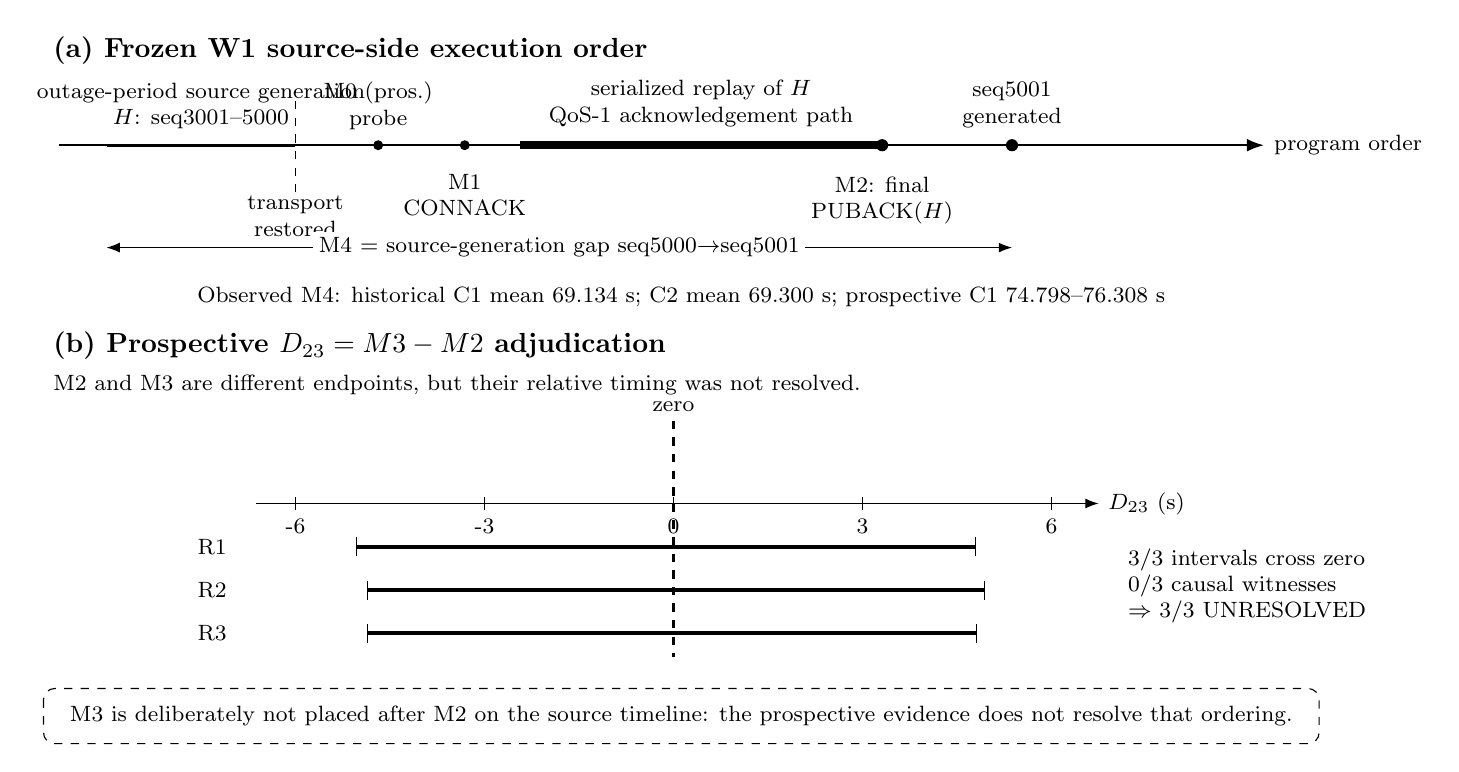
\begin{tikzpicture}[font=\footnotesize,>=Latex,x=1cm,y=1cm]
  \node[anchor=west,font=\bfseries] at (0,3.55) {(a) Frozen W1 source-side execution order};
  \draw[->,line width=0.7pt] (0.2,2.35) -- (15.5,2.35) node[right] {program order};
  \draw[line width=1.1pt] (0.8,2.35) -- (3.2,2.35);
  \node[align=center] at (2.0,2.85) {outage-period source generation\\$H$: seq3001--5000};
  \draw[dashed] (3.2,1.75) -- (3.2,3.05);
  \node[align=center] at (3.2,1.45) {transport\\restored};
  \fill (4.25,2.35) circle (1.8pt);
  \node[align=center] at (4.25,2.85) {M0 (pros.)\\probe};
  \fill (5.35,2.35) circle (1.8pt);
  \node[align=center] at (5.35,1.72) {M1\\CONNACK};
  \draw[line width=3pt] (6.05,2.35) -- (10.65,2.35);
  \node[align=center] at (8.35,2.88) {serialized replay of $H$\\QoS-1 acknowledgement path};
  \fill (10.65,2.35) circle (2.2pt);
  \node[align=center] at (10.65,1.65) {M2: final\\PUBACK($H$)};
  \fill (12.3,2.35) circle (2.2pt);
  \node[align=center] at (12.3,2.86) {seq5001\\generated};
  \draw[<->] (0.8,1.05) -- (12.3,1.05);
  \node[fill=white,inner sep=2pt] at (6.55,1.05) {M4 = source-generation gap seq5000$\rightarrow$seq5001};
  \node[align=center] at (8.1,0.42) {Observed M4: historical C1 mean 69.134~s; C2 mean 69.300~s; prospective C1 74.798--76.308~s};

  \node[anchor=west,font=\bfseries] at (0,-0.20) {(b) Prospective $D_{23}=M3-M2$ adjudication};
  \node[anchor=west,align=left] at (0,-0.70) {M2 and M3 are different endpoints, but their relative timing was not resolved.};
  \coordinate (O) at (8,-2.2);
  \draw[->] (2.7,-2.2) -- (13.4,-2.2) node[right] {$D_{23}$ (s)};
  \foreach \x/\lab in {-6/-6,-3/-3,0/0,3/3,6/6} {
    \draw ($(O)+(\x*0.8,0.08)$) -- ($(O)+(\x*0.8,-0.08)$);
    \node[below] at ($(O)+(\x*0.8,-0.08)$) {\lab};
  }
  \draw[dashed,line width=0.8pt] (8,-1.15) -- (8,-4.15);
  \node[above] at (8,-1.15) {zero};
  \foreach \y/\name/\lo/\hi in {-2.75/R1/-5.038/4.801,-3.30/R2/-4.857/4.932,-3.85/R3/-4.858/4.815} {
    \node[anchor=east] at (2.45,\y) {\name};
    \draw[line width=1.4pt] ($(O)+(\lo*0.8,\y+2.2)$) -- ($(O)+(\hi*0.8,\y+2.2)$);
    \draw ($(O)+(\lo*0.8,\y+2.08)$) -- ($(O)+(\lo*0.8,\y+2.32)$);
    \draw ($(O)+(\hi*0.8,\y+2.08)$) -- ($(O)+(\hi*0.8,\y+2.32)$);
  }
  \node[anchor=west,align=left] at (13.65,-3.25) {3/3 intervals cross zero\\0/3 causal witnesses\\$\Rightarrow$ 3/3 UNRESOLVED};

  \draw[rounded corners,dashed] (0,-4.55) rectangle (16.2,-5.25);
  \node[align=center] at (8.1,-4.9) {M3 is deliberately not placed after M2 on the source timeline: the prospective evidence does not resolve that ordering.};
\end{tikzpicture}%
}
\caption{Evidence-faithful recovery measurement view. (a) shows only source-side program order that is fixed by the W1 implementation; the M4 gap is measured from generation of seq5000 to generation of seq5001. (b) shows the three conservative prospective $D_{23}$ intervals, each crossing zero. The figure therefore does not encode an unsupported M2-before-M3 ordering.}
\label{fig:recoveryview}
\end{figure*}

None of the three runs produced the same-receiver causal witness: after the receiver observed sequence 5001, it did not subsequently observe a previously missing member of $H$. The conservative $D_{23}=M3-M2$ intervals also crossed zero in all three runs. Consequently, no run was positive under either frozen route, and all three were classified UNRESOLVED. The Stage-A adjudication was therefore 0/3 positive and \texttt{NOT\_CONFIRMED\_STOP}; the protocol did not authorize Stage B.

This result is negative but informative. It does not show that M2 and M3 are equal, because the clock uncertainty leaves their relative timing unresolved. It also does not support the earlier claim that M2 materially precedes M3 by a repeated measurable interval. The prospective evidence instead establishes the appropriate claim ceiling: broker-side PUBACK closure and receiver-side historical completion remain semantically different endpoints, but a repeated positive temporal separation was not resolved in this campaign.

\subsection{POWDER: bounded cross-layer, failure-domain, and stale-carryover evidence}

The POWDER transition experiments show that lower-layer and application-layer indicators did not move in lockstep in the preserved profile. In E1R4 at 51~dB, ICMP lost 30\% of 20 probes while MQTT receiver reconciliation remained complete at 20/20. At 52~dB, the same ascending run showed 60\% ICMP loss and 13/20 unique MQTT records. In descending E2, 52~dB produced 65\% ICMP loss and 11/20 MQTT records, whereas at 51~dB ICMP loss fell to 10\% while MQTT again reached 20/20. Across the three E3 cycles at 52~dB, MQTT completeness varied among 60\%, 25\%, and 55\%, while ICMP loss varied among 80\%, 65\%, and 70\%. These measurements support an experiment-specific transition region with substantial cycle variability, not a deterministic 52~dB threshold.

Recovery observations also depended on the affected mechanism and declared endpoint. E10-A is retained as censored because no recovery was observed in the preserved window. In E10-B, RF restoration plus UE restart yielded action-begin-to-first-MQTT-publish of 6.063318~s and action-begin-to-first-ping of 6.609430~s; publish-to-CORE receipt was 0.060172~s. In E10-C-B, the preserved CORE-related sequence yielded RF-restore-to-first-ping of 29.247733~s and RF-restore-to-first-MQTT-publish of 29.248129~s. E10-D supports only the upper bound $\leq 10.908749$~s from action begin to a manually initiated successful publish. These quantities describe different interventions and endpoints and are not combined.

E8 provides a complementary isolation result: during the broker interruption, the UE and reverse CORE ping paths remained 20/20 while MQTT records 21--40 were absent; final unique delivery was 40/60 after duplicate recovery sends were preserved in the evidence. This shows that application-layer MQTT service loss can coexist with a healthy tested LTE ping path in that control.

Finally, the E3 cycle-3 receiver trace at 52~dB contained a bounded M5 event: sequences 251--255 arrived before the older sequence 231. Because this ordering is established on the same receiver clock, it does not require cross-host synchronization. It supports only an existence claim that stale carryover can survive restoration in a physical test instance. No occurrence rate or general MQTT prevalence is inferred.

\subsection{Cross-evidence synthesis}

The three evidence classes support different parts of the measurement argument. Historical FIT shows repeated W1 replay-associated generation blackout together with eventual 10,000/10,000 completeness. Prospective FIT reproduces the continuity cost at roughly 75--76~s while directly testing M2 and M3; the temporal separation question remains unresolved rather than positive. POWDER shows that lower-layer health, MQTT delivery, failure-domain recovery, timing semantics, and receiver ordering can disagree in bounded physical observations.

The synthesis is therefore methodological rather than statistical. Table~\ref{tab:coverage} shows that endpoint coverage differs by campaign, while Fig.~\ref{fig:recoveryview} separates known W1 source-side program order from the unresolved M2/M3 temporal relation. A single value called recovery time would erase distinctions among path restoration, MQTT session restoration, broker-side acknowledgement closure, receiver completeness, continuity of current data generation, and stale historical carryover. The evidence supports measuring these observables separately. It does not support a pooled cross-testbed recovery effect, a universal durability--freshness law, or a repeated empirical M2-before-M3 claim.

\section{Discussion}
\label{sec:discussion}

\subsection{Completeness and continuity are different properties}

The strongest repeated FIT result is a measured implementation consequence, not an architecture ranking, a receiver-latency estimate, or a claim of an emergent generic MQTT phenomenon. In the tested W1 implementation, the code path serially drains the historical backlog before generation of sequence 5001; the experiments quantify the resulting continuity cost. Eventual receiver completeness was preserved while generation of the first record after the historical set was suspended for approximately 69~s in the historical campaign and 75--76~s in the prospective campaign. The two campaigns are reported separately because their instrumentation and execution conditions differ.

This result is implementation-specific and structurally consistent with W1's serialized execution order. A different scheduler could interleave current and historical traffic, prioritize current state, or apply another policy entirely. The data therefore do not support a generic statement that MQTT durability harms freshness. They show that replay policy is part of the service behavior that must be measured. Direct comparison of alternative replay schedulers, backlog-size scaling, replay concurrency, and broker-throughput sensitivity is outside the bounded claim tested here and is reserved for future work.

\subsection{What the prospective negative result changes}

M2 and M3 remain semantically different endpoints: the final broker-side QoS-1 acknowledgement for $H$ is not the same event as the receiver having observed every member of $H$. However, semantic distinction is not evidence of a material time separation. The prospective Stage-A campaign was designed to test that stronger proposition and produced 0/3 positive runs. No same-receiver causal witness occurred, and every conservative $D_{23}$ interval crossed zero. The correct conclusion is therefore UNRESOLVED, not that M2 equals M3 and not that M2 repeatedly precedes M3.

Retaining this negative result is important for the measurement argument. A recovery methodology should be able to say that a proposed distinction was not temporally resolved under the available evidence. Treating uncertainty as a positive result would reproduce the endpoint error that motivated the revival.

\subsection{Failure domain and evidence semantics}

The POWDER observations show why recovery measurements require a named domain, action, endpoint, and timing class. E10-A is censored because no recovery endpoint was observed in the preserved window. E10-B and E10-C-B provide exact measurements for their declared interventions and endpoints. E10-D is only an upper bound. These values are all valid, but they are not samples of one common recovery-latency variable.

The same principle appears across layers. E1R4 at 51~dB shows degraded ICMP while receiver-observed MQTT completeness remained 20/20. E8 shows MQTT loss during a broker interruption while the tested LTE ping path remained healthy. E3 cycle 3 supplies a same-receiver stale-carryover event. These observations do not imply that one layer is generally more robust than another; they show that a single health indicator cannot represent every state relevant to a telemetry service.

\subsection{Recovery declaration matrix}

Table~\ref{tab:declaration} converts the observable taxonomy into an operational reporting discipline. It does not define a new protocol state machine; it records what each evidence class can and cannot close.

\begin{table*}[t]
\centering
\small
\caption{Recovery declaration matrix derived from the M0--M5 measurement boundary.}
\label{tab:declaration}
\begin{tabular}{p{0.20\textwidth}p{0.31\textwidth}p{0.41\textwidth}}
\toprule
\textbf{Observed state} & \textbf{Evidence authority} & \textbf{Permitted interpretation} \\
\midrule
Path restored & Successful declared M0 user-plane probe & The tested path is reachable; MQTT session and receiver state remain separate questions. \\
MQTT session restored & Successful M1 CONNACK & The publisher session is restored; historical receiver completeness is not established. \\
Broker-side historical closure & Final M2 PUBACK covering $H$ & The publisher-to-broker QoS-1 obligation for $H$ is closed; subscriber completion is not established by this event alone. \\
Receiver historical state complete & M3 identity reconciliation for every unique member of $H$ & Historical-state completion may be declared for the named receiver and set. \\
Current-data continuity characterized & M4 source-generation timing & Replay-induced continuity cost can be reported without reinterpreting it as M3 latency. \\
Stale carryover / ordering observed & M5 same-receiver arrival order & An ordering event can be declared for that trace; prevalence is not implied. \\
Recovery not observed & Observation window closes before the declared endpoint & Censored; no scalar latency is assigned. \\
Recovery transition not timestamped exactly & First observed success follows an interval with unknown exact transition & Report an upper bound rather than an exact latency. \\
\bottomrule
\end{tabular}
\end{table*}

\subsection{Engineering implication}

For telemetry monitoring, the practical implication is to expose the event being measured rather than reporting a generic recovered flag. A system may legitimately report path restoration or session restoration while separately tracking historical-state completion and continuity of current measurements. Conversely, a receiver-side completeness check can close a historical-state objective without saying anything about whether current generation was uninterrupted. This decomposition permits incident reports, dashboards, and recovery experiments to remain precise without requiring a new MQTT wire protocol.

\section{Threats to Validity}
\label{sec:threats}

The principal validity threat is historical endpoint instrumentation. The original FIT instrumentation did not timestamp exact receiver-side M3 completion and used a field named backlog drain that actually terminated at sender-side QoS-1 acknowledgement closure. The revival corrects that interpretation and does not reconstruct an unmeasured historical M3 latency.

The prospective campaign improves endpoint instrumentation but does not eliminate clock uncertainty. Cross-host timing was bounded conservatively; all three $D_{23}$ intervals crossed zero, and no same-receiver causal witness occurred. Consequently, 0/3 positive runs do not establish that M2 and M3 are equal. They establish only that a repeated positive separation was not resolved under the frozen decision rule.

External validity is intentionally narrow. The W1 replay behavior depends on the tested implementation, backlog size, workload, broker/client software, hardware, and outage treatment. The approximately 69~s historical and 75--76~s prospective generation gaps must not be generalized to MQTT deployments that use different replay or scheduling policies. B0 is intentionally non-durable and therefore serves only as a mechanism-isolation control; it is not a strongest-available durable MQTT comparator.

The FIT run is the scientific unit. The 10,000 record identities within each run are used for deterministic reconciliation and are not treated as independent experimental samples. Historical architecture--condition cells contain three run-level replicates, and prospective Stage A contains three valid run-level replicates. The study therefore reports bounded repeated engineering observations and descriptive run values rather than population reliability estimates, message-level confidence intervals, or hypothesis tests.

FIT and POWDER are heterogeneous testbeds with deliberately different evidence roles. Their measurements are not pooled and agreement between them is not treated as replication. POWDER attenuation values characterize only the preserved profile; 52~dB is not a universal threshold. The stale-carryover observation is a single bounded physical trace and supports existence only, not frequency or prevalence.

Recovery timing on POWDER is also endpoint-specific. Exact E10-B and E10-C-B measurements, censored E10-A evidence, and the E10-D upper bound are not interchangeable. Finally, the experiments are controlled testbed studies rather than field or production validation; they do not establish agronomic, industrial-process, safety-critical, or deployment-wide reliability claims.

\section{Reproducibility and Data Availability}
\label{sec:repro}

The manuscript is accompanied by a sanitized reviewer-facing reproducibility supplement under
\path{manuscript/revival_2026-09-22/supplement_r7fr3/}.
The supplement contains: (i) a campaign execution-configuration matrix, (ii) the exact public code-authority manifest, (iii) the pre/post clock-bound procedure, (iv) the historical/prospective treatment definitions, (v) the raw-evidence preservation boundary, and (vi) a standard-library self-check. The package intentionally excludes credentials, SSH private keys, private Drive identifiers, and protected raw archives.

The principal public code authorities used for the prospective campaign are the frozen runner \texttt{fit\_runner\_py35.py}, the sidecar instrumentation wrapper \texttt{fit\_runner\_q0\_instrumented\_py35.py}, the receiver stamp stream, the scored Stage-A loop, and the deterministic per-run and aggregate adjudicators. The supplement records their Git blob identities so that reviewer inspection targets the code that actually underlies the reported result rather than a later reconstruction.

The prospective scored FIT Stage-A raw archive remains the immutable measurement authority. It contains the three run analyses, aggregate Stage-A verdict, bootstrap evidence, workflow console, adjudication console, and an internal SHA-256 manifest. Its frozen archive identity is:
\begin{center}
\small\texttt{5b52005e48d8987091c447186eb392618}\\
\texttt{24f32df15653c3d2773a031b062d4a2}
\end{center}
The 6,881,643-byte archive contains 127 entries and was copied to three durable storage locations; each copy was re-downloaded and verified against the same SHA-256 digest. Historical FIT and POWDER claims remain traceable through the project's frozen reconstruction tables, forensic trace maps, immutable archive hashes, and receiver-side identity reconciliation.

A complete live FIT rerun requires an authorized FIT IoT-LAB account and current platform availability. The submission package therefore supports source-level audit and deterministic re-adjudication without publishing account secrets. Exact receiver-side \texttt{mosquitto\_sub} versions were not captured in the frozen FIT metadata and are explicitly left unreported rather than inferred. The final public archival DOI, if assigned later, is an editorial release artifact and is not invented here.

\section{Conclusion}
\label{sec:conclusion}

This study reconstructs telemetry recovery as a set of experimentally distinct observables rather than one generic recovery time. In the tested W1 implementation, serialized historical replay preserved eventual receiver completeness but repeatedly suspended generation of the first post-backlog record for tens of seconds: approximately 69~s in the historical FIT campaign and 75--76~s in the separate prospective campaign. The experiments therefore quantify the magnitude and repeatability of a continuity cost implied by that serialized code path; they do not establish a universal MQTT effect.

The prospective experiment directly instrumented broker-side PUBACK closure and receiver historical-state completion, yet 0/3 runs produced a causal or clock-resolved positive separation. The M2-to-M3 interval therefore remains unresolved rather than demonstrated. POWDER contributes complementary bounded evidence that lower-layer health, application delivery, recovery endpoint semantics, and receiver ordering can diverge across physical failure scenarios, including one stale-carryover trace.

The resulting contribution is an evidence discipline: name the failure domain, define the observable endpoint, preserve exact/censored/upper-bound semantics, and distinguish historical completeness from current-data continuity. The study does not introduce a new persistence architecture and does not pool heterogeneous testbeds into a global reliability claim.

\section*{Acknowledgment}
The author acknowledges FIT IoT-LAB for access to its experimental IoT infrastructure and POWDER for access to its wireless experimentation platform.

\section*{Funding}
This work received no external research funding.

\section*{Conflict of Interest}
The author declares that he has no known competing financial interests or personal relationships that could have appeared to influence the work reported in this paper.
\begin{thebibliography}{14}

\bibitem{mqtt5}
A.~Banks, E.~Briggs, K.~Borgendale, and R.~Gupta, Eds.,
``MQTT Version 5.0,'' OASIS Standard, Mar. 2019.

\bibitem{emqtt}
Y.~Im and M.~Lim,
``E-MQTT: End-to-end synchronous and asynchronous communication mechanisms in MQTT protocol,''
\emph{Appl. Sci.}, vol.~13, no.~22, Art.~no.~12419, 2023,
doi: 10.3390/app132212419.

\bibitem{jesus2025}
B.~Jesus, F.~Lins, and N.~Laranjeiro,
``An approach to assess robustness of MQTT-based IoT systems,''
\emph{Internet Things}, vol.~31, Art.~no.~101590, 2025,
doi: 10.1016/j.iot.2025.101590.

\bibitem{gaspar2026}
L.~Gaspar, J.~N.~C.~Faria, M.~Domingues, F.~Fama, L.~Martins, and D.~Portugal,
``The price of reliability: Stress-testing MQTT in practical IoT communications,''
\emph{IEEE Internet Things Mag.}, 2026,
doi: 10.1109/MIOT.2026.3681190.

\bibitem{neagu2026}
M.~Neagu, C.~M.~Serban, A.~Hangan, and G.~Sebestyen,
``Digital twins at the edge: A high-availability framework for resilient data processing in IoT sensor networks,''
\emph{Future Internet}, vol.~18, no.~3, Art.~no.~137, 2026,
doi: 10.3390/fi18030137.

\bibitem{kang2026}
S.~Kang, C.~Li, C.~G.~Brinton, A.~Eryilmaz, and N.~B.~Shroff,
``Balancing current and historical state information in remote tracking systems: A randomized update approach,''
\emph{IEEE/ACM Trans. Netw.}, vol.~34, pp.~4377--4386, 2026,
doi: 10.1109/TON.2026.3673496.

\bibitem{fitlab}
C.~Adjih, E.~Baccelli, E.~Fleury, G.~Harter, N.~Mitton, T.~Noel, R.~Pissard-Gibollet, F.~Saint-Marcel, G.~Schreiner, J.~Vandaele, and T.~Watteyne,
``FIT IoT-LAB: A large scale open experimental IoT testbed,''
in \emph{Proc. 2nd IEEE World Forum Internet Things (WF-IoT)}, Milan, Italy, 2015, pp.~459--464,
doi: 10.1109/WF-IoT.2015.7389098.

\bibitem{powder}
J.~Breen, A.~Buffmire, J.~Duerig, K.~Dutt, E.~Eide, A.~Ghosh, M.~Hibler, D.~Johnson, S.~K.~Kasera, E.~Lewis, D.~Maas, C.~Martin, A.~Orange, N.~Patwari, D.~Reading, R.~Ricci, D.~Schurig, L.~B.~Stoller, A.~Todd, J.~Van~der~Merwe, K.~Webb, and G.~Wong,
``Powder: Platform for Open Wireless Data-driven Experimental Research,''
\emph{Comput. Netw.}, vol.~197, Art.~no.~108281, 2021,
doi: 10.1016/j.comnet.2021.108281.


\bibitem{mohammed2026resilient}
A.~Mohammed, R.~S.~S.~Singh, S.~Aslam, and T.~T.~Yew,
``A resilient MQTT-based architecture for real-time solar photovoltaic monitoring,''
\emph{Int. J. Intell. Eng. Syst.}, vol.~19, no.~5, pp.~320--334, 2026,
doi: 10.22266/ijies2026.0531.19.

\bibitem{mohammed2026scalable}
A.~Mohammed, R.~S.~S.~Singh, S.~Aslam, and Y.~C.~Wong,
``A scalable MQTT-based edge IoT architecture for real-time distributed solar PV panel monitoring,''
\emph{Eng. Technol. Appl. Sci. Res.}, vol.~16, no.~3, pp.~36014--36024, 2026,
doi: 10.48084/etasr.16945.

\bibitem{chen2020}
F.~Chen, P.~Liu, J.~Zhu, S.~Gao, Y.~Zhang, M.~Duan, Y.~Wang, K.~Hwang, and H.~Gao,
``Improving topic-based data exchanges among IoT devices,''
\emph{Security Commun. Netw.}, vol.~2020, pp.~1--14, 2020,
doi: 10.1155/2020/8884924.

\bibitem{sochor2021}
H.~Sochor, F.~Ferrarotti, and R.~Ramler,
``An automated evaluation of broker compatibility for the Message Queuing Telemetry Transport protocol,''
\emph{J. Softw. Evol. Process}, vol.~35, no.~7, 2021,
doi: 10.1002/smr.2410.

\bibitem{nawaz2019}
M.~S.~Nawaz, M.~Sun, B.~Shahzad, M.~I.~U.~Lali, T.~Umer, and S.~Wan,
``Quality of service in IoT protocol as designs and its verification in PVS,''
\emph{Trans. Emerg. Telecommun. Technol.}, vol.~33, no.~8, 2019,
doi: 10.1002/ett.3742.

\bibitem{kamoun2024}
K.~Kamoun, F.~Hmissi, S.~Ouni, and S.~Ouni,
``Improvement of MQTT semantic to minimize data flow in IoT platforms based on distributed brokers,''
\emph{Trans. Emerg. Telecommun. Technol.}, vol.~35, no.~2, 2024,
doi: 10.1002/ett.4945.
\end{thebibliography}

\end{document}
